\documentclass[hyphens]{beamer}

\usepackage[utf8]{inputenc}
\usepackage[ngerman]{babel}

\usepackage{array}
\usepackage{tabularx}
\newcolumntype{Z}{>{\centering\let\newline\\\arraybackslash\hspace{0pt}}p{0.65\textwidth}}

\usepackage{amssymb}
\usepackage{pifont}
\newcommand{\xmark}{\ding{55}}
\usepackage{svg}

\usetheme[progressbar=frametitle,block=fill]{metropolis}

\setbeamertemplate{section in toc}[sections numbered]
\setbeamertemplate{subsection in toc}[subsections numbered]
\setbeamertemplate{caption}{\raggedright\insertcaption\par}

\defbeamertemplate{subsubsection in toc}{subsubsections numbered}
{\leavevmode\leftskip=3em%
 \rlap{\hskip-3em\inserttocsectionnumber.\inserttocsubsectionnumber.\inserttocsubsubsectionnumber}%
 \inserttocsubsubsection\par}

\setbeamertemplate{subsubsection in toc}[subsubsections numbered]

\begin{document}
  \title[Gerät zur Schlaganfall-Rehabilitation]{Entwicklung eines Gamification-basierten Biofeedback-Unterstützungs- und Motivationsgeräts zur Rehabilitation von Schlaganfall-Patienten \\ \small{- Zwischenstandsverteidigung -}}
  \author[Lukas Rost]{Lukas Rost  \\ \and \emph{Fachbetreuer:} Johannes Süpke \\ \and \emph{Außenbetreuer:} Hannes Weichel (topdev GmbH)}
  \institute[ASGspez]{Spezialschulteil des staatlichen Gymnasiums "'Albert Schweitzer"' Erfurt}
  \date{27. Juni 2018}

 \begin{frame}
 \titlepage
 \end{frame}

  \begin{frame}
\begin{figure}
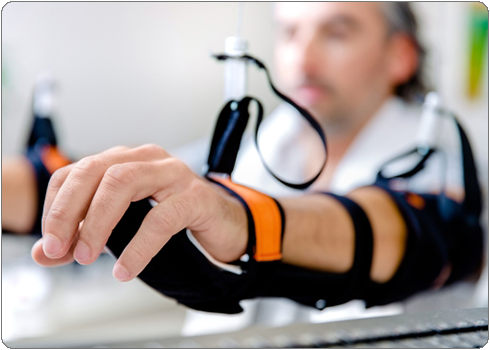
\includegraphics[scale=0.6]{../Themenverteidigung/pics/einleit1}
  \caption{Therapiegerät für Armlähmungen}
\end{figure}
 \end{frame}

 \begin{frame}
 \titlepage
 \end{frame}

 \begin{frame}{Gliederung}
 \tableofcontents
 \end{frame}

 \section{Änderungen des Konzepts}
 \begin{frame}{Änderungen des Konzepts}
 \begin{columns}[T]
 \begin{column}{0.33\textwidth}
 \begin{figure}
 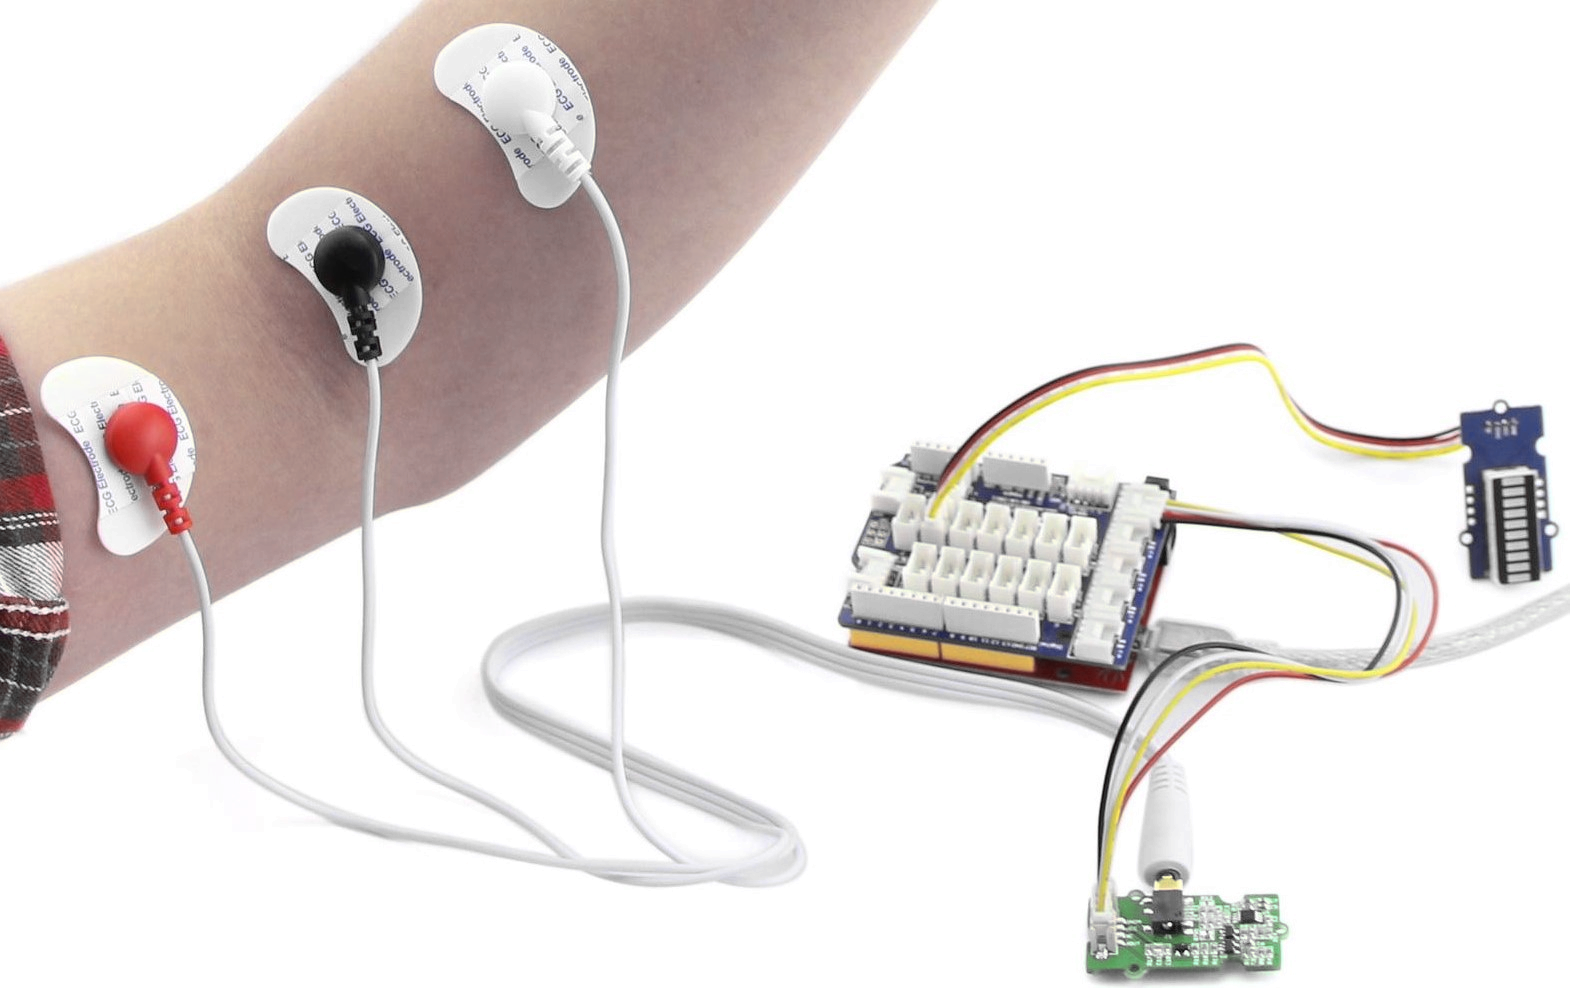
\includegraphics[scale=0.08]{img/grove-emg.png}
\caption{EMG-Sensor}
 \end{figure}
 \end{column}
 \pause
 \begin{column}{0.33\textwidth}
 \begin{figure}
 \hspace{6pt}
 \includesvg[scale=1.5]{img/Kotlin-logo.svg}
 \caption{Kotlin-Logo}
 \end{figure}
 \end{column}
 \pause
 \begin{column}{0.34\textwidth}
 \begin{figure}
 \vspace{10pt}
 \includesvg[scale=0.1]{img/OpenGLES.svg}
 \caption{OpenGL-Logo}
 \end{figure}
 \end{column}
 \end{columns}
 \end{frame}


 \section{Darstellung des Arbeitsstands}
 \begin{frame}{Darstellung des Arbeitsstands}
 \begin{itemize}
 \item Fertigstellung der Theoriekapitel und der Kapitel zum Mikrocontroller
 \end{itemize}
 \begin{figure}
 
\includegraphics[scale=0.4]{img/kapitel}
 \caption{Ausschnitt aus einem Kapitel}
 \end{figure}
 \end{frame}

 \begin{frame}{Darstellung des Arbeitsstands}
 \begin{itemize}
 \item erfolgreicher Entwurf und Aufbau der Schaltung für den Mikrocontroller
 \item erfolgreiche Implementierung eines funktionsfähigen Programms auf dem Mikrocontroller
 \end{itemize}
 \begin{figure}
 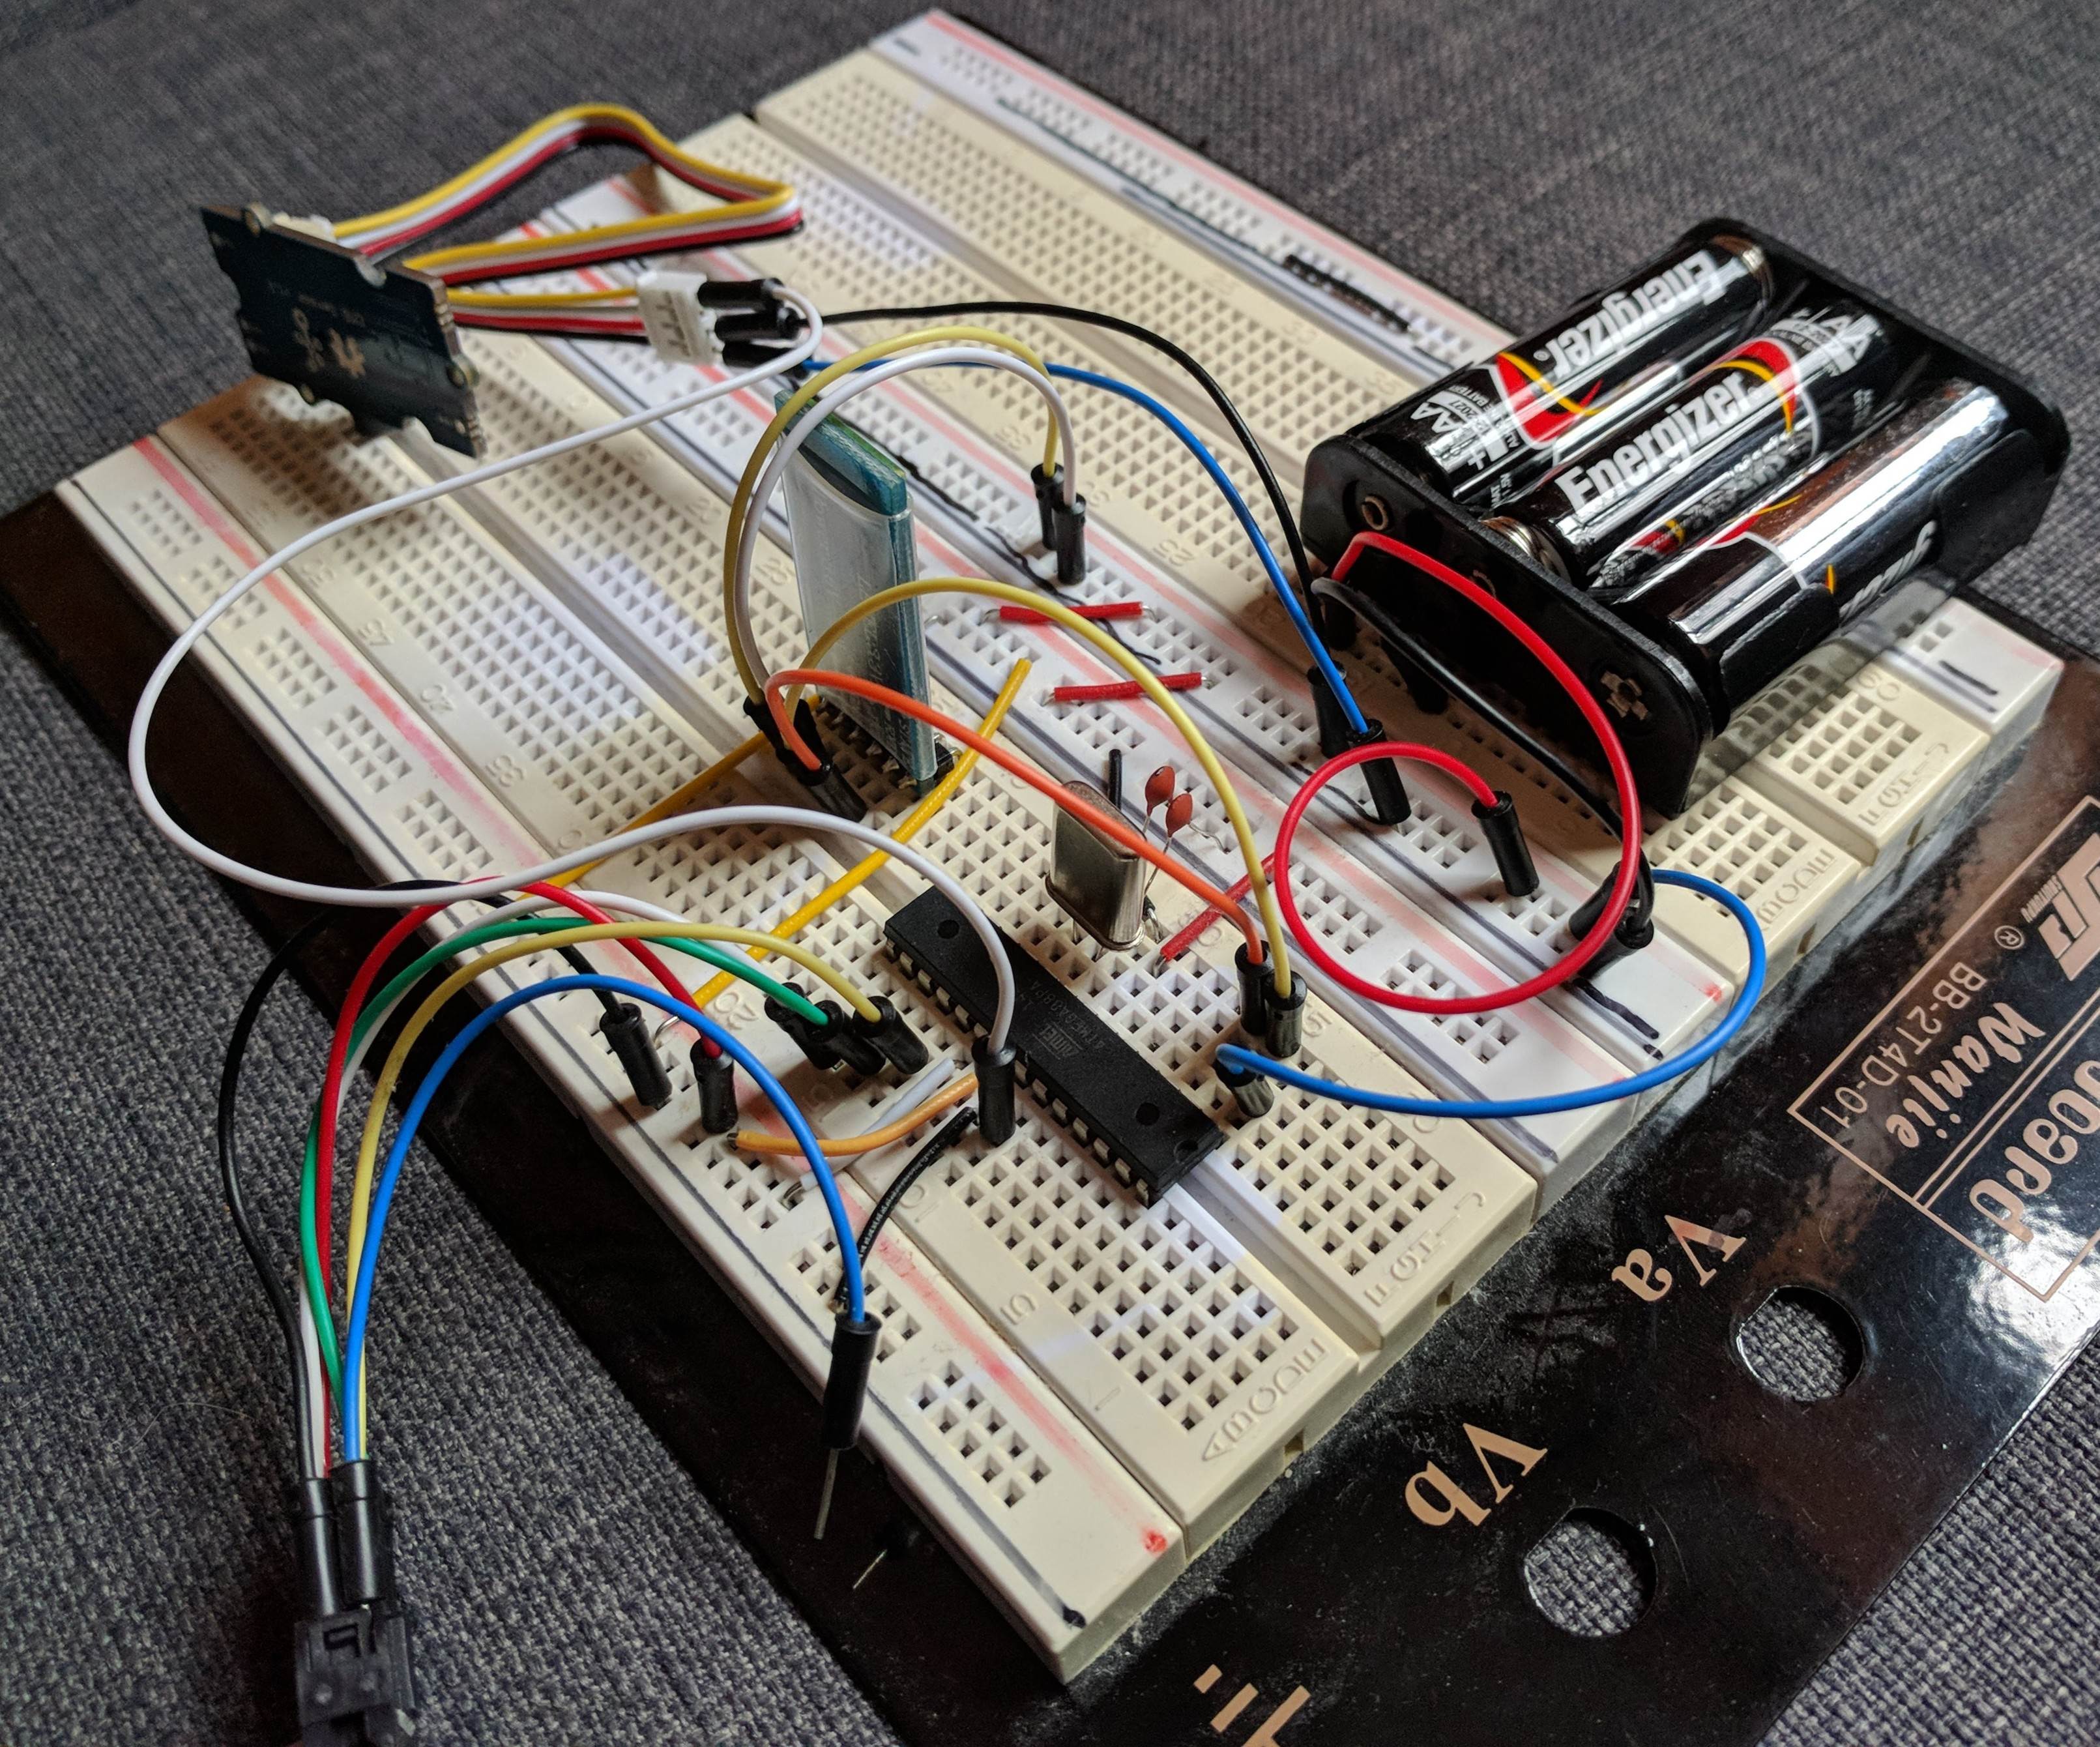
\includegraphics[scale=0.04]{img/IMG_20180624_182058}
 \caption{Mikrocontroller mit Schaltung}
 \end{figure}
 \end{frame}

 \begin{frame}{Darstellung des Arbeitsstands}
 \begin{itemize}
 \item Erstellung eines Feinkonzeptes zu Aufbau und Struktur der Begleit-App
 \item Erstellung eines Designprototypen der App
 \end{itemize}
 \begin{columns}[T]
  \begin{column}{0.5\textwidth}
  \begin{figure}
  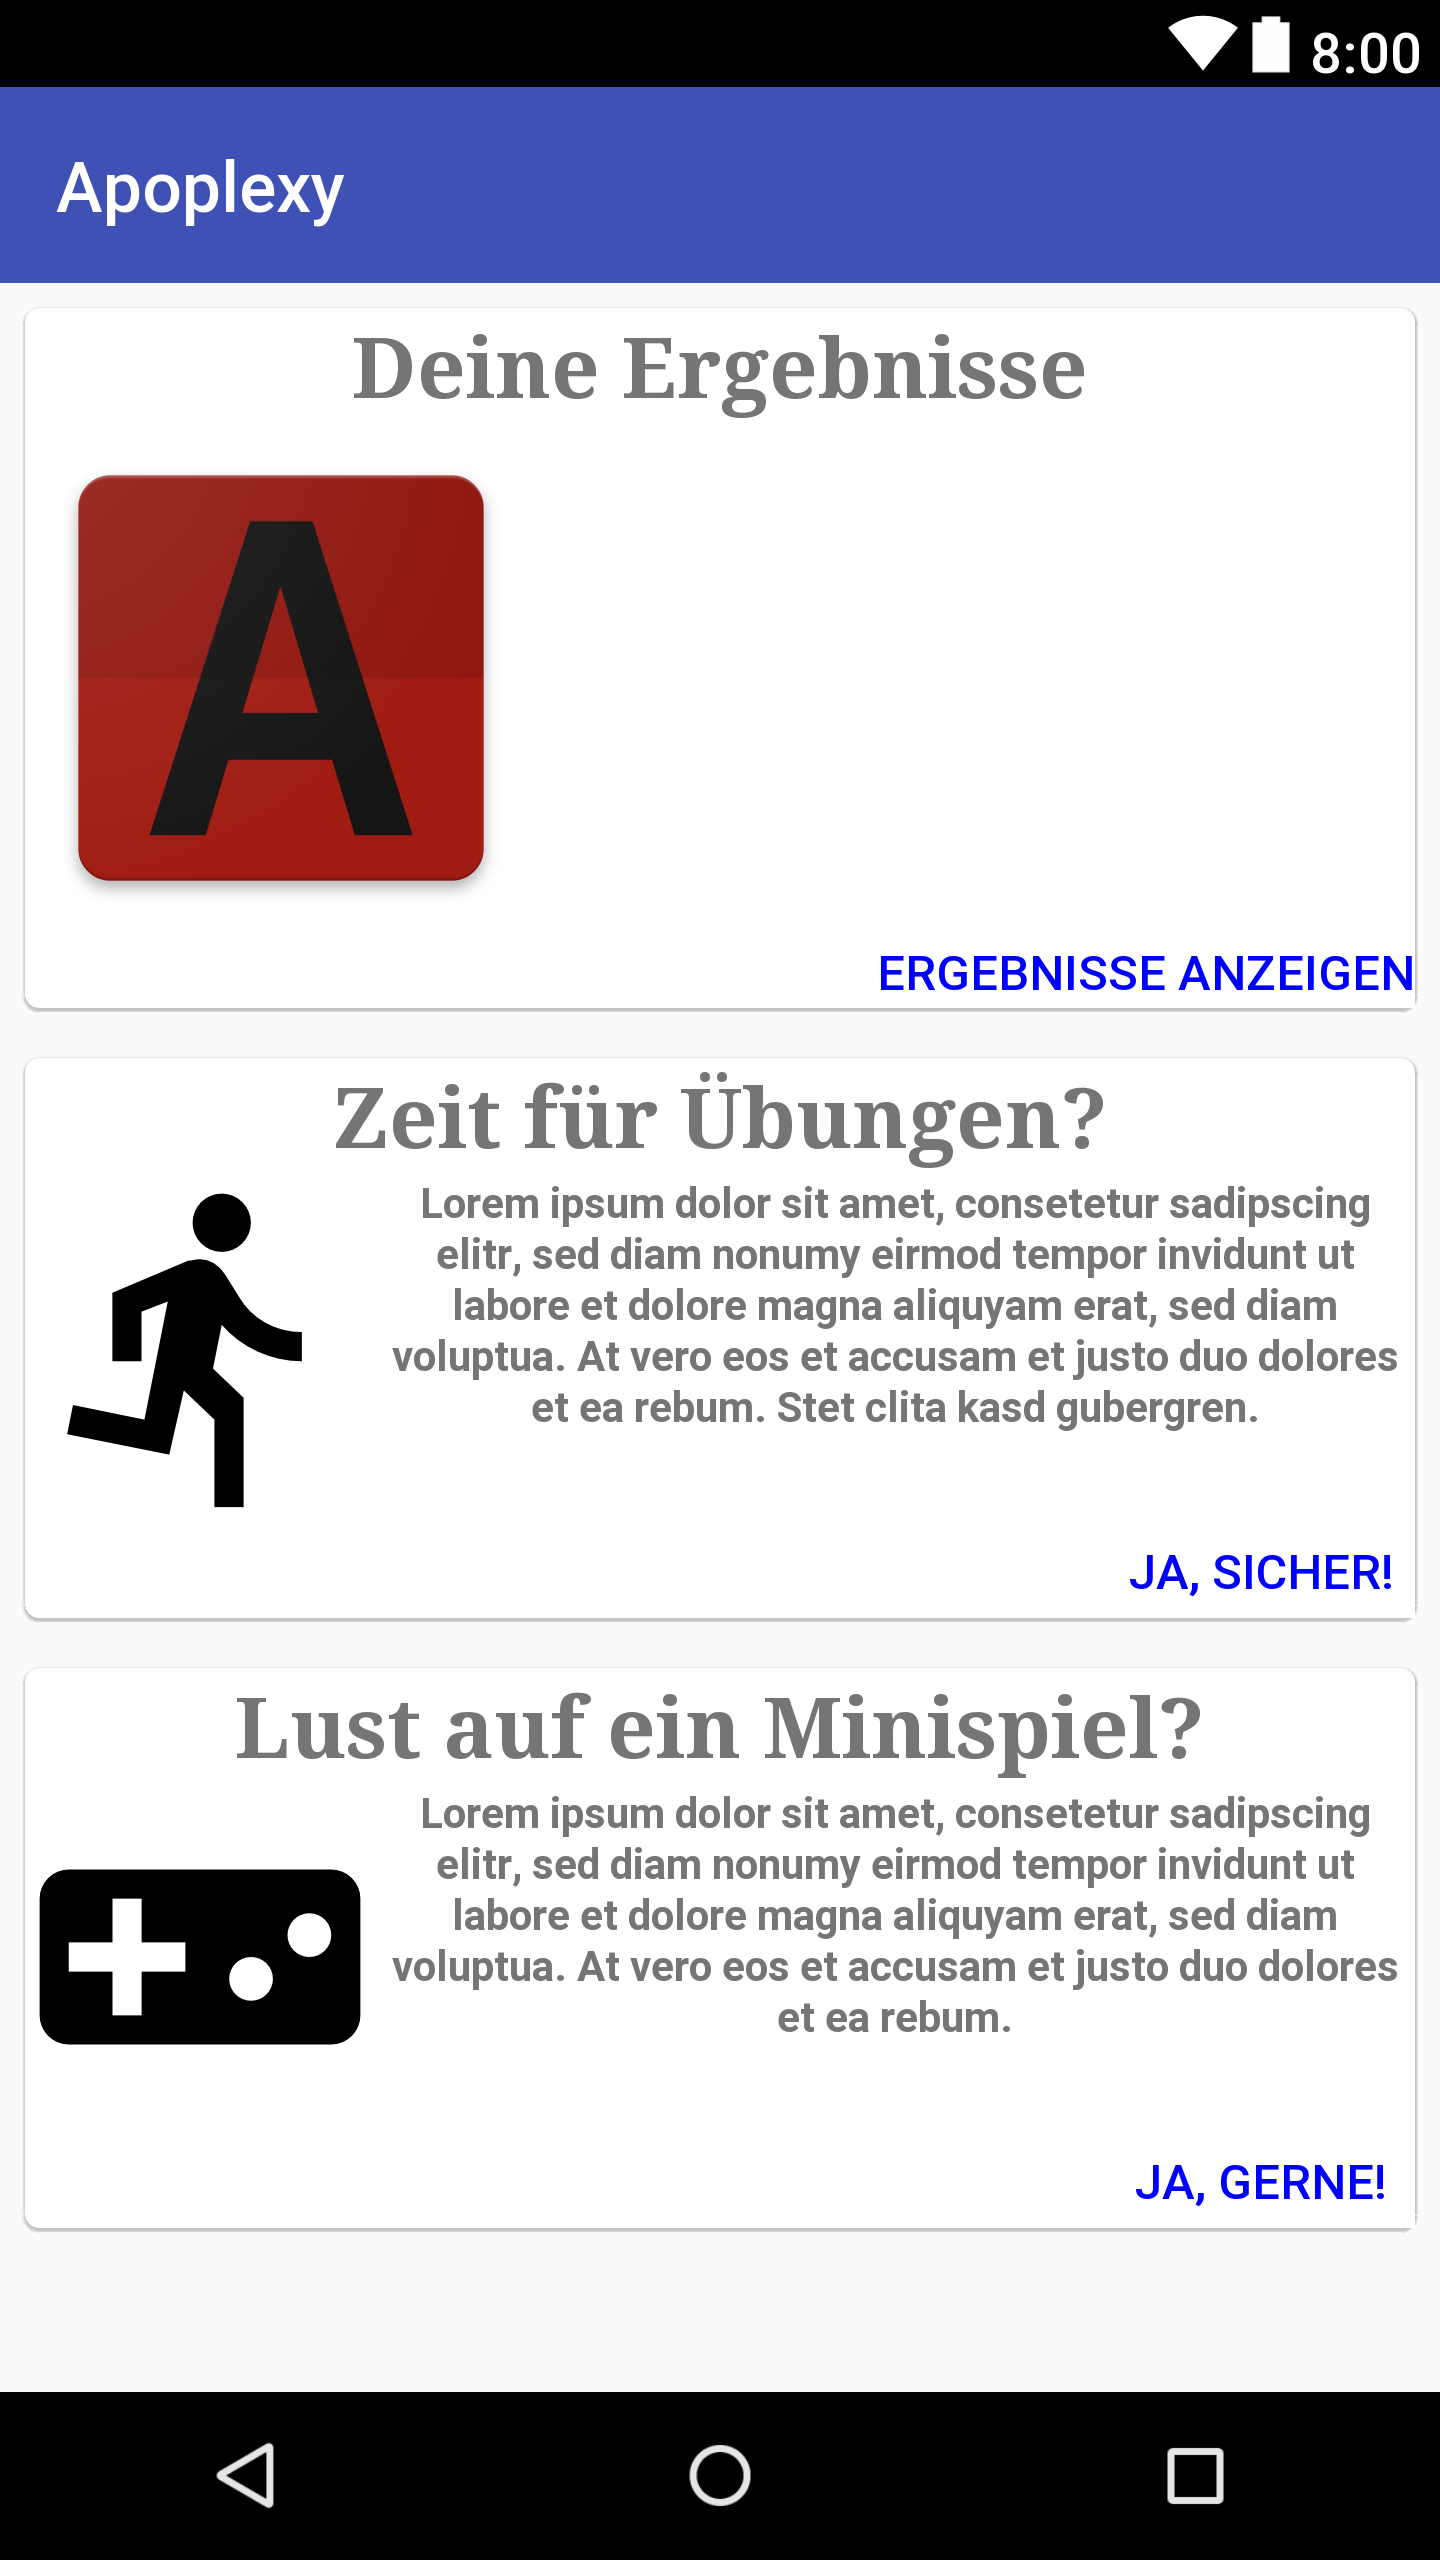
\includegraphics[scale=0.05]{img/layout-home}
  \caption{Start-Activity der App}
  \end{figure}
  \end{column}
  \begin{column}{0.5\textwidth}
  \begin{figure}
  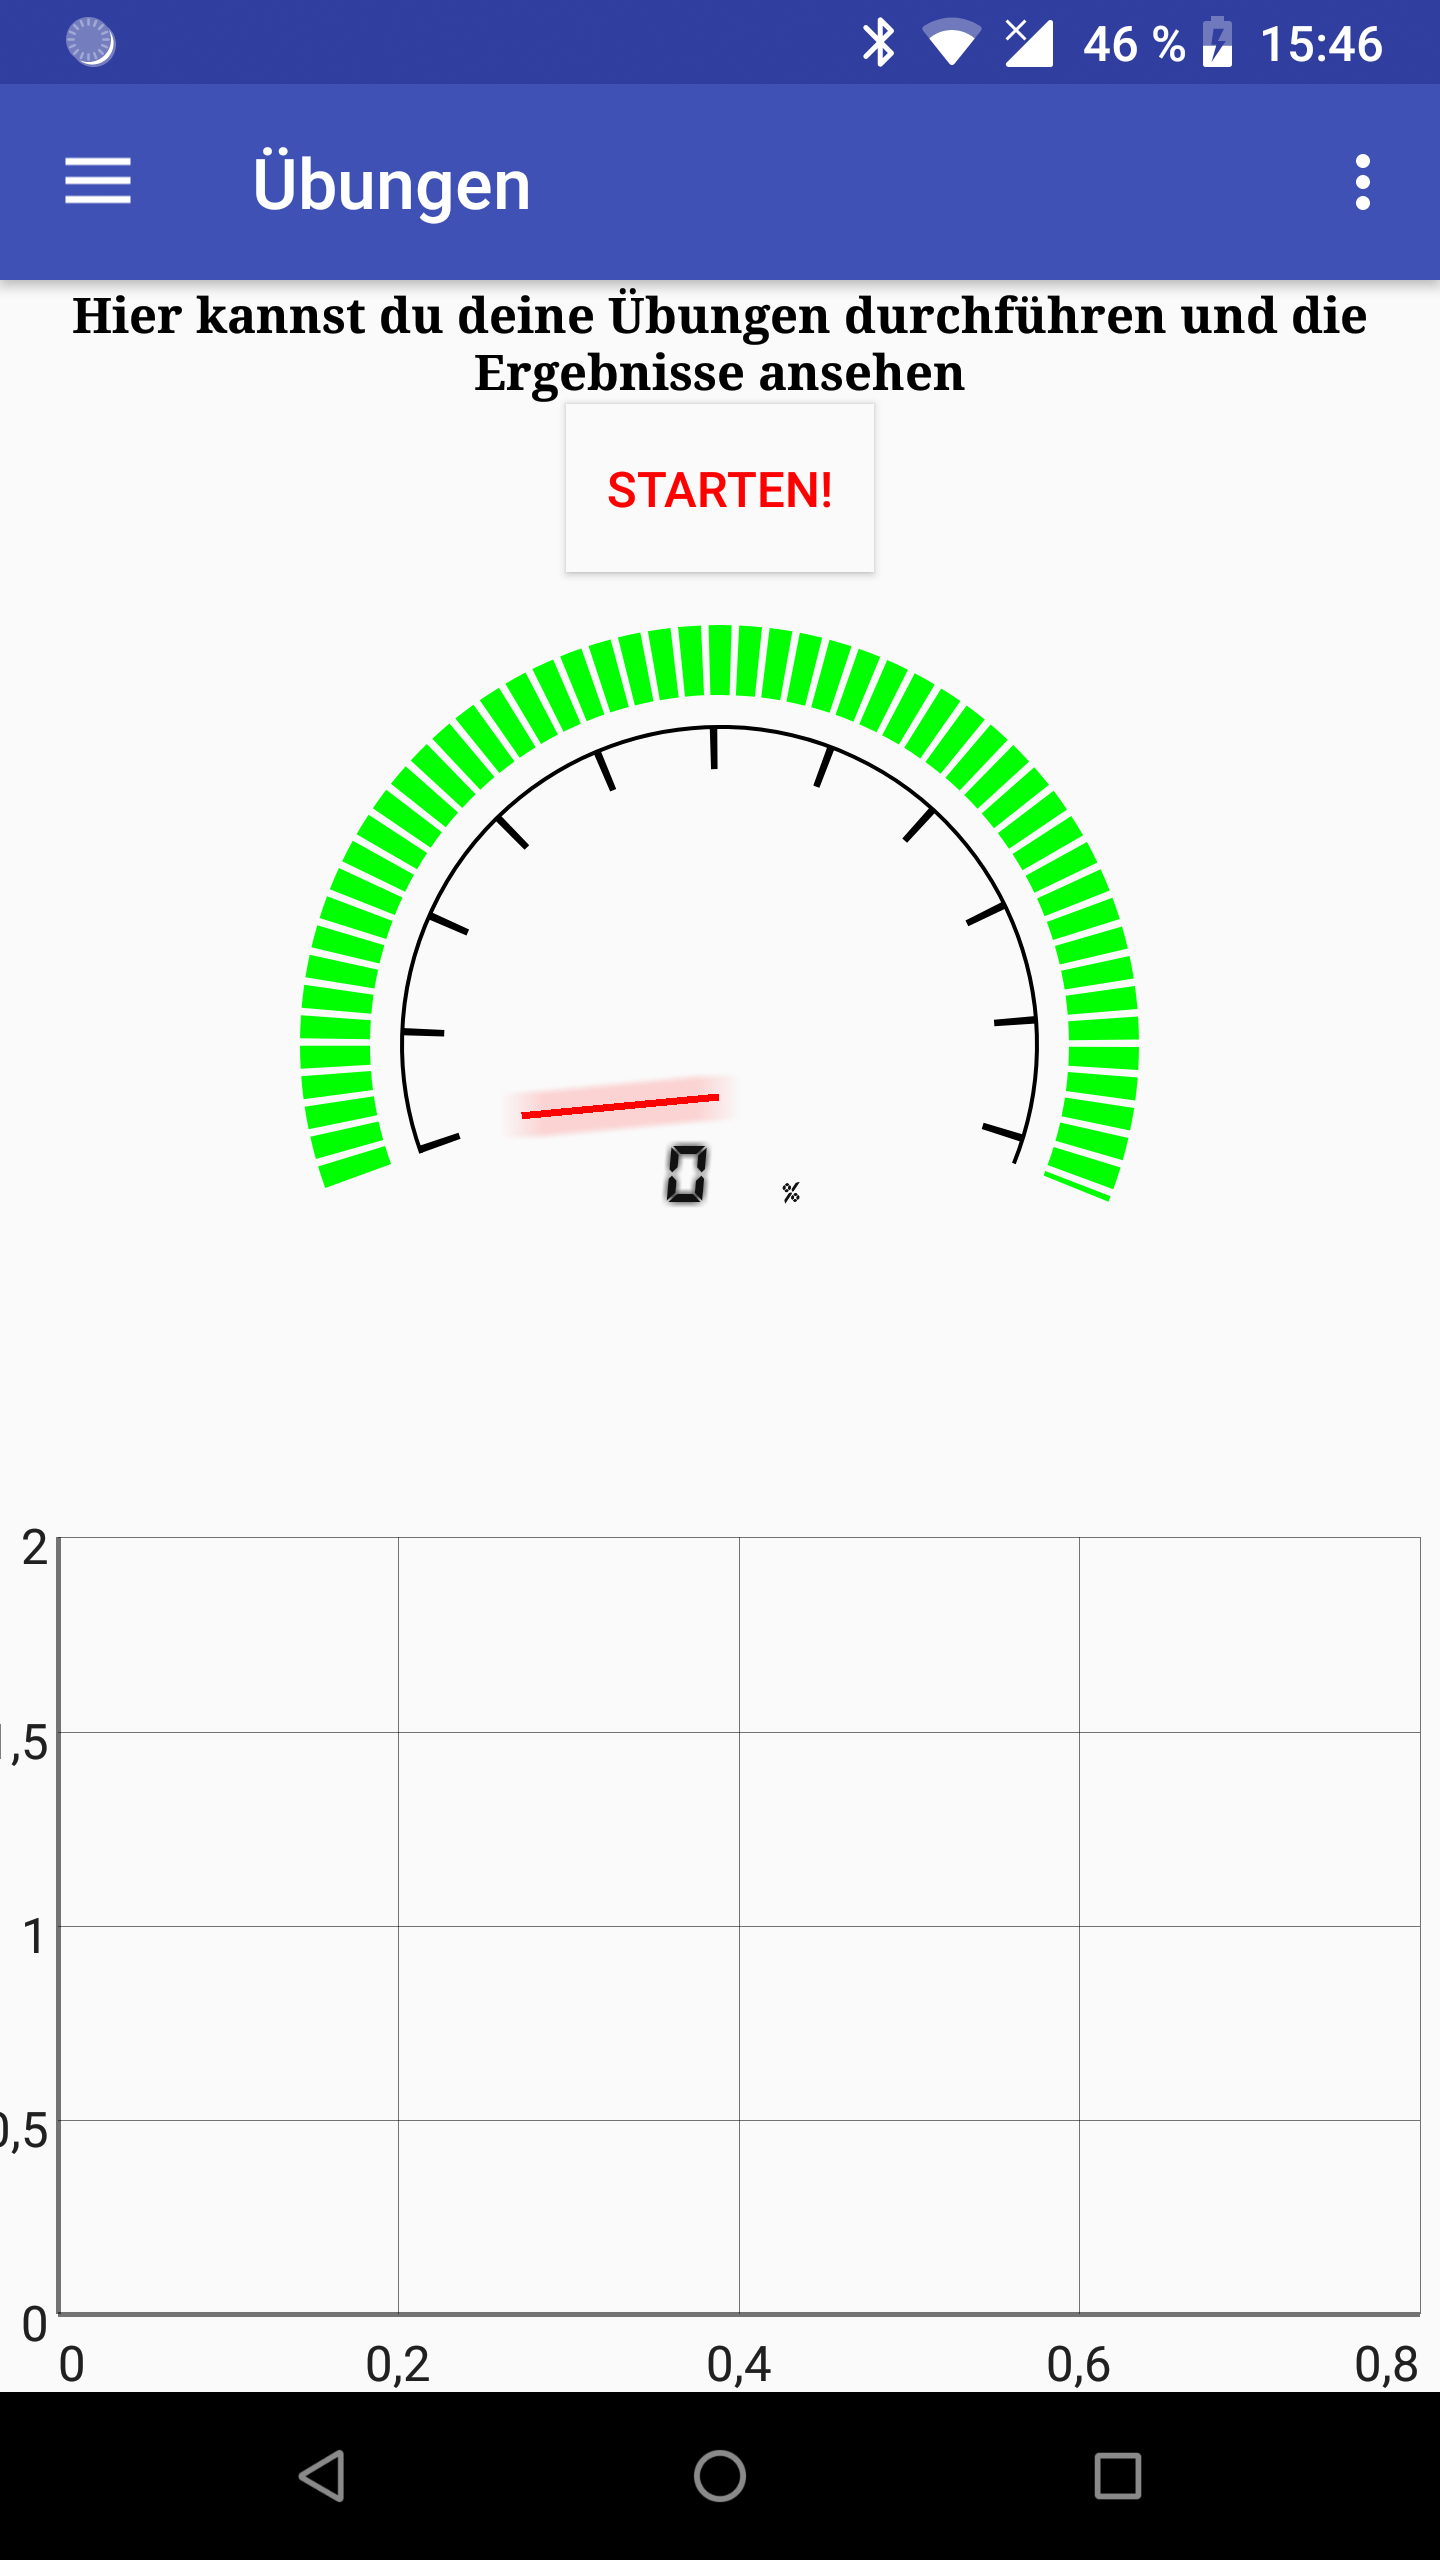
\includegraphics[scale=0.05]{img/layout_exercise}
  \caption{Übungs-Activity der App}
  \end{figure}
  \end{column}
 \end{columns}
 \end{frame}

 \section{Kritische Reflexion des Erreichten und der Arbeitsmethoden}
 \begin{frame}{Kritische Reflexion des Erreichten}
 \begin{itemize}[<+->]
 \item bessere Ausarbeitung des Konzepts vor der Themen- verteidigung wäre wünschenswert gewesen (weniger Änderungen nötig)
 \item Arbeitsfortschritt bis zur Zwischenstandsverteidigung hätte schneller sein sollen
 \begin{itemize}
   \item[-$>$] aber: langwierigeres Literaturstudium und Fehlersuche (Debugging)
 \end{itemize}
 \item grundsätzlich guter Arbeitsfortschritt, innerhalb des Zeitplans
 \item bisherige Vorhaben erfolgreich fertiggestellt
 \item weitere Ziele sehr wahrscheinlich bis zur Abgabe der Arbeit erreichbar
 \end{itemize}
 \end{frame}

 \section{Weitere Vorhaben}
 \begin{frame}{Weitere Vorhaben}
 \begin{flushleft}
 \begin{table}
 \begin{small}
 \begin{tabularx}{\columnwidth}{p{0.3\textwidth}|Z}
 \hline
 \textbf{Zeitraum bis...} & \textbf{Vorhaben} \\ \hline
 August 2018 & Entwicklung der Android-App \\ \hline
 Oktober 2018 & Entwicklung der integrierten Minispiels \\ \hline
 Dezember 2018 & Verfassen der weiteren Kapitel \\ \hline
 März 2019 & ggf. Praxistest \\ \hline
 März 2019 & Vorbereitung des Kolloquiums \\ \hline
 2019 & Teilnahme an \glqq Jugend forscht\grqq \\ \hline
 \end{tabularx}
 \end{small}
 \end{table}
 \end{flushleft}
 \end{frame}

 \begin{frame}{Bildquellen}
 \begin{itemize}
 \item \small{\url{https://raw.githubusercontent.com/SeeedDocument/Grove-EMG_Detector/master/img/Emg_connect.jpg}}
 \item \small{\url{https://upload.wikimedia.org/wikipedia/commons/7/74/Kotlin-logo.svg}}
 \item \small{\url{https://upload.wikimedia.org/wikipedia/commons/1/17/OpenGL_ES_Nov14.svg}}
 \item \small{selbst erstellt}
 \end{itemize}
 \end{frame}

 \begin{frame}
 \titlepage
 \end{frame}

\end{document}
